%
% AEVO_Florian-Wilhelm Florian Wilhelm
% Erstellt am 07.12.2013
%
% Bauen mit dem beiliegenden Makefile

\documentclass[11pt,a4paper,notitlepage,ngerman]{article}

% Deutsch mit neuer Rechtschreibung
\usepackage[ngerman]{babel}

% Umlaute direkt eingeben http://www.jr-x.de/publikationen/latex/tipps/besonderheiten.html
% Hatte hier ursprünglich "latin1" als Option, das ging aber nicht. Hängt wohl von der Codierung des Dokumentes ab.
\usepackage[utf8]{inputenc} 

% Einbinden von Grafiken
\usepackage{graphicx}

% Setzen der Eigenschaften der erzeugten PDF-Datei
\usepackage[pdftex,
    pdfauthor={Florian Wilhelm},
    pdfsubject={AEVO Florian Wilhelm},
    pdftitle={AEVO Florian Wilhelm},    
    pdfproducer={Latex with hyperref},
    pdfcreator={pdflatex}]{hyperref}

\begin{document}

\renewcommand\footnotemark{} % http://tex.stackexchange.com/questions/14865/using-thanks-and-footnote-without-without-numbering-mark-and-line
\renewcommand\footnoterule{}

\title{Schriftliche Ausarbeitung zur AEVO-Prüfung\\Thema:\\Systematisches Vorgehen zum Beheben eines Software-Fehlers}
\author{Florian Wilhelm\footnote{{\large Ich versichere, diese Ausarbeitung selbst erstellt zu haben: \underline{\hspace{3cm}} (Datum) \underline{\hspace{3cm}} (Unterschrift)  }}}
\date{7. Januar 2014}
\maketitle


\tableofcontents
\newpage

\section{Ausgangslage}

\subsection{Ausbildungsbetrieb}

Der Ausbildungsbetrieb, die \emph{Unternehmensberatung Müller Informatik GmbH},
ist ein mittelständisches Systemhaus, das seinen Kunden
das volle Spektrum an Leistungen anbietet, die diese im IT-Bereich benötigen.
Die meisten Kunden sind im sozialen Bereich tätig, einige davon sind auch
Stadtwerke. Die \emph{UMI GmbH} hat circa 300 Mitarbeiter an ihrem Stammsitz in Bruchsal,
zusätzlich hat sie noch einige kleinere Vertriebsstellen in Deutschland und Europa
verteilt, in denen ein paar Dutzend Menschen beschäftigt sind. 

\subsection{Eigene Person}

Ich bin Ausbildungsleiter der Abteilung \emph{Programmentwicklung}, welche für
die Entwicklung, Anpassung, Wartung, Qualitätssicherung und den 3rd-Level-Support
verantwortlich ist.

\subsubsection{Der Auszubildende}

Der Auszubildende, Max Schmidt, ist seit September 2013 im Unternehmen. Er ist
19 Jahre alt und hat nach seiner mittleren Reife ein zweijähriges Berufskolleg
absolviert, womit er eine Fachhochschulreife erworben hat. Trotzdem entschied er sich
den Weg einer dualen Berufsausbildung zu gehen, da ihm weniger an der grauen
Theorie liegt als daran, endlich selbst aktiv Projekte mitzugestalten.

Er lernt den Beruf des \emph{Fachinformatikers} in der Fachrichtung \emph{Anwendungsentwicklung}.
Einige Vorkenntnisse brachte er schon mit, da er seit seiner Realschulzeit
hobbymäßig programmiert. 

\subsubsection{Problemstellung}

Bei einem Kunden ist seit der Aktualisierung der Software ein Problem aufgetreten,
welches unter bestimmten (noch nicht näher bekannten) Umständen dazu führt,
dass das Programm langsam arbeitet. Nach einem Neustart des Computers funktioniert
es wieder wie gewohnt. Eigentlich müssten solche Fehler vor der Auslieferung von der Qualitätssicherung entdeckt werden, doch dieser scheint 
\glqq durchgerutscht\grqq{} zu sein.

Die Kundenhotline, bei der der Mitarbeiter des Kunden zuerst gelandet ist, kann
an dieser Stelle nicht weiterhelfen und wendet sich an die Abteilung 
\emph{Programmentwicklung}.

Das Ziel ist es, dem Auszubildenden beizubringen, wie man in einer solchen Situation
systematisch vorgeht, um in kurzer Zeit und hoher Qualität eine Lösung für das Problem
zu erstellen.

Da der Fehler nicht dazu führt, dass Daten verloren gehen und es auch mit dem
Fehler möglich ist, mit dem Programm zu arbeiten, ist es kein besonders dringendes
Problem. Deshalb ist es gut dafür geeignet, dem Auszubildenden am realen Kundenfall
die Gelegenheit zum Lernen zu geben. Trotzdem erwartet der Kunde zu Recht, dass
sein Problem in angemessener Zeit behoben wird.

\section{Lernziele}

Die Lernziele sind entnommen aus dem \emph{Ausbildungsrahmenplan Fachinformatiker / Fachinformatikerin} der IHK.

\subsection{Richtlernziel}

\emph{Kundenspezifische Anpassung und Softwarepflege (§ 10 Abs. 2 Nr. 9.1)}

\subsection{Groblernziel}

\emph{d) Fehler beseitigen}

\subsection{Feinlernziele}

\subsubsection{Kognitiver Bereich}

Der Auszubildende ist nach der Unterweisung in der Lage \ldots

\begin{itemize}
  \item{den Umgang mit den im Betrieb verwendeten Softwareentwicklungswerkzeugen}
  \item{eine systematische Vorgehensweise zur Fehlersuche}
  \item{Vorgehensweisen zum logischen Eingrenzen der Fehlerquelle durch Ausschließen von irreführenden Informationen}
\end{itemize}

zu kennen.

\subsubsection{Affektiver Bereich}

Der Auszubildende ist nach der Unterweisung in der Lage \ldots

\begin{itemize}
  \item{die gebotene Sorgfalt im Umgang mit Kundeninformationen}
  \item{Einhaltung von Datenschutzbestimmungen}
  \item{Einhaltung des Urheberrechts am Quellcode der Software}
\end{itemize}

zu beachten.

\subsubsection{Psychomotorischer Bereich}

In dieser Unterweisung wird der psychomotorische Bereich nicht angesprochen.

\section{Schlüsselqualifikationen}

Qualifikationen, die diese Unterweisung besonders fördern sind \emph{logisches Denken},
\emph{Problemlösefähigkeit}, \emph{Handlungswissen} und \emph{sorgfältiges Arbeiten}.

\section{Die gewählte (Unterweisungs-)Methode}

Als Unterweisungsmethode wird ein modifiziertes \emph{Handlungsorientiertes Lehrgespräch}
verwendet. Diese Methode besteht aus vier Schritten:

\begin{enumerate}
  \item{Informationsinput durch Ausbilder}
  \item{Einbeziehung von Erfahrungen des Azubi}
  \item{Sammeln der Fakten}
  \item{Zusammenfassen und gegebenenfalls Ergänzen durch weitere Informationen}  
\end{enumerate}

Die Modifikation besteht darin, zwischen dem dritten und vierten Schritt
eine ca. vierstündige Eigenarbeitsphase des Auszubildenden einzuplanen. So soll
ihm genügend Zeit gegeben werden eigene Erfahrungen zu machen und sich eine
eigenständige Arbeitsweise anzueignen. Es soll dabei jedoch verhindert werden,
dass der Auszubildende sich überfordert und alleingelassen fühlt, deshalb
darf er selbstverständlich Fragen stellen wenn er über einen längeren Zeitraum
keinen Fortschritt macht.

\section{Alternative Methoden}

Alternativ hätten die \emph{Vier-Stufen-Methode} und die \emph{Projektmethode}
zur Verfügung gestanden.

Die \emph{Vier-Stufen-Methode} wurde nicht ausgewählt, weil sie zu sehr darauf
fixiert ist, feste Arbeitsabläufe stur zu wiederholen. In dieser Ausbildungssituation
ist es aber notwendig, kognitiv zu handeln.

Die \emph{Projektmethode} wurde nicht ausgewählt, weil sie dem natürlichen
Arbeitsablauf in der gegebenen Situation nicht so gut entspricht wie das
\emph{Handlungsorientierte Lehrgespräch}. Sie ist eher geeignet für
Ausbildungssituationen, in denen zum Beispiel ein neues Programmmodul entwickelt
werden muss.

\section{Verlaufsplan}

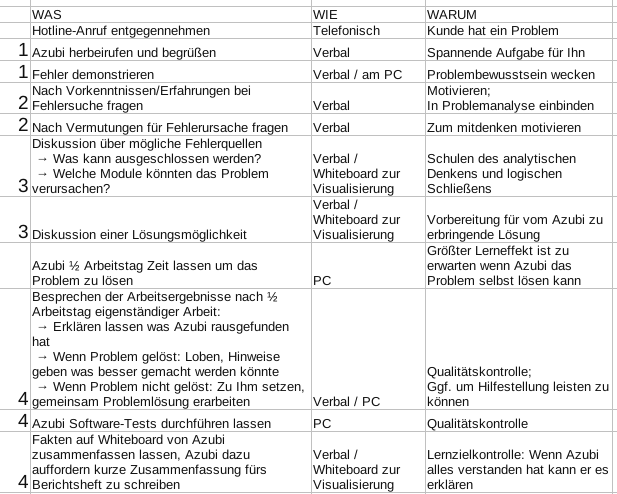
\includegraphics[scale=0.6]{pic/verlaufsplan.png}

\section{Lernerfolgskontrolle}

Das Lernziel ist erreicht, wenn der Auszubildende in der Lage ist, selbstständig
Fehlerberichte von der Hotline entgegenzunehmen, diese reproduzierbar nachzuvollziehen,
die fehlerhafte Stelle im Quellcode ausfindig machen, den Fehler zu beheben und
die Richtigkeit seiner Änderung durch Software-Tests nachzuvollziehen.
Dabei muss er alle seine Arbeitsschritte vorschriftsmäßig dokumentieren.

Um das erreichen des Lernziels zu überprüfen werden dem Auszubildenden nach
und nach komplexere Teilaufgaben übertragen. Dabei wird er aufgefordert,
eigenständig an der Lösung der Aufgaben zu arbeiten, für Rückfragen und eine
abschließende Qualitätskontrolle steht der Ausbilder zur Verfügung.

Außerdem fasst der Azubi die gewonnenen Erkenntnisse auf dem Whiteboard und
für sein Berichtsheft zusammen. Gelingt ihm das, so ist sichergestellt,
dass er etwas gelernt hat.

\end{document}
